\documentclass{article}

\usepackage[utf8]{inputenc}

\usepackage{amsmath}
\usepackage{graphicx}
\usepackage{amssymb}
\usepackage{float}

\setlength{\parskip}{\baselineskip}%
\setlength{\parindent}{0pt}%

\begin{document}

\title{Boundary Layers}
\author{lwp26 }
\date{October 2022}
\maketitle

\section{Abstract}

\section{Introduction}

% Aims, Objectives and context

\subsection{Aims}

\begin{itemize}
\item To gather flow data and calculate velocity profiles for both laminar and turbulant flows.
\item To analyse and compare the flow velocity profiles of laminar and turbulant flows to gain an understanding of boundary layers
\item To calculate errors from tolerances of components and compare these to the measured values
\end{itemize}

\section{Methodology}

% Summary of theory and information to reproduce
\subsection{Flow velocity profiles}
The velocity profiles were determined using a wind tunnel with 2 manometers. One manometer's pitot probe was placed far away from the wall and was used to measure $V_\infty$ The other manometer's pitot probe's position was varied to record $V$ at $x$ mm from the wall.

From Bernouli's equation
\begin{equation}
    p_0 - p = \frac{1}{2}\rho_l u^2 = \rho_l g \Delta h sin \theta
\end{equation}
After rearanging for flow velocity, $u$, equation (1) becomes
\begin{equation}
    u = \sqrt{2 g \Delta h sin \theta}
\end{equation}
Which means the ratio of flow velocities becomes
\begin{equation}
    r_u = \frac{u}{U_\infty} = \sqrt{\frac{\Delta h}{\Delta h_\infty}}
\end{equation}
The Reynolds number of a flow is a dimensionless quantity used to distuinguish between laminar and turbulant flow.
It can be calculated using the equation below
\begin{equation}
    R_e = \frac{\rho_l u L}{\mu}
\end{equation}
At high Reynolds numbers, typically $R_e > 10^5$ for a flat plate, the flow transitions from laminar to turbulant.

The momentum flux is the rate of momentum transfer per unit area. It is given by
\begin{equation}
    \dot{M} = \int_0^\infty (U_{\infty} - u) \rho u dy = \int_0^\infty \rho U_{\infty}^2 \left( 1 - \frac{u}{U_{\infty}} \right) \left( \frac{u}{U_{\infty}} \right) dy
\end{equation}

\subsection{Drag coefficient of spheres}

The drag coefficient of an aerofoil is a dimensionless quantity used to quantify how aerodynamic an object is.
\begin{equation}
    C_D = \frac{F_D}{\frac{1}{2}\rho_l U^2 L}
\end{equation}
For the case of falling vertically in a fluid the drag force $F_D$ can be calculated using the weight and upthrust as seen below
\begin{equation}
    C_D = \frac{mg - \rho V g}{\frac{1}{2}\rho_l U^2 L}
\end{equation}

\section{Results}


\subsection{Flow profiles}

\begin{figure}[H]
\centering
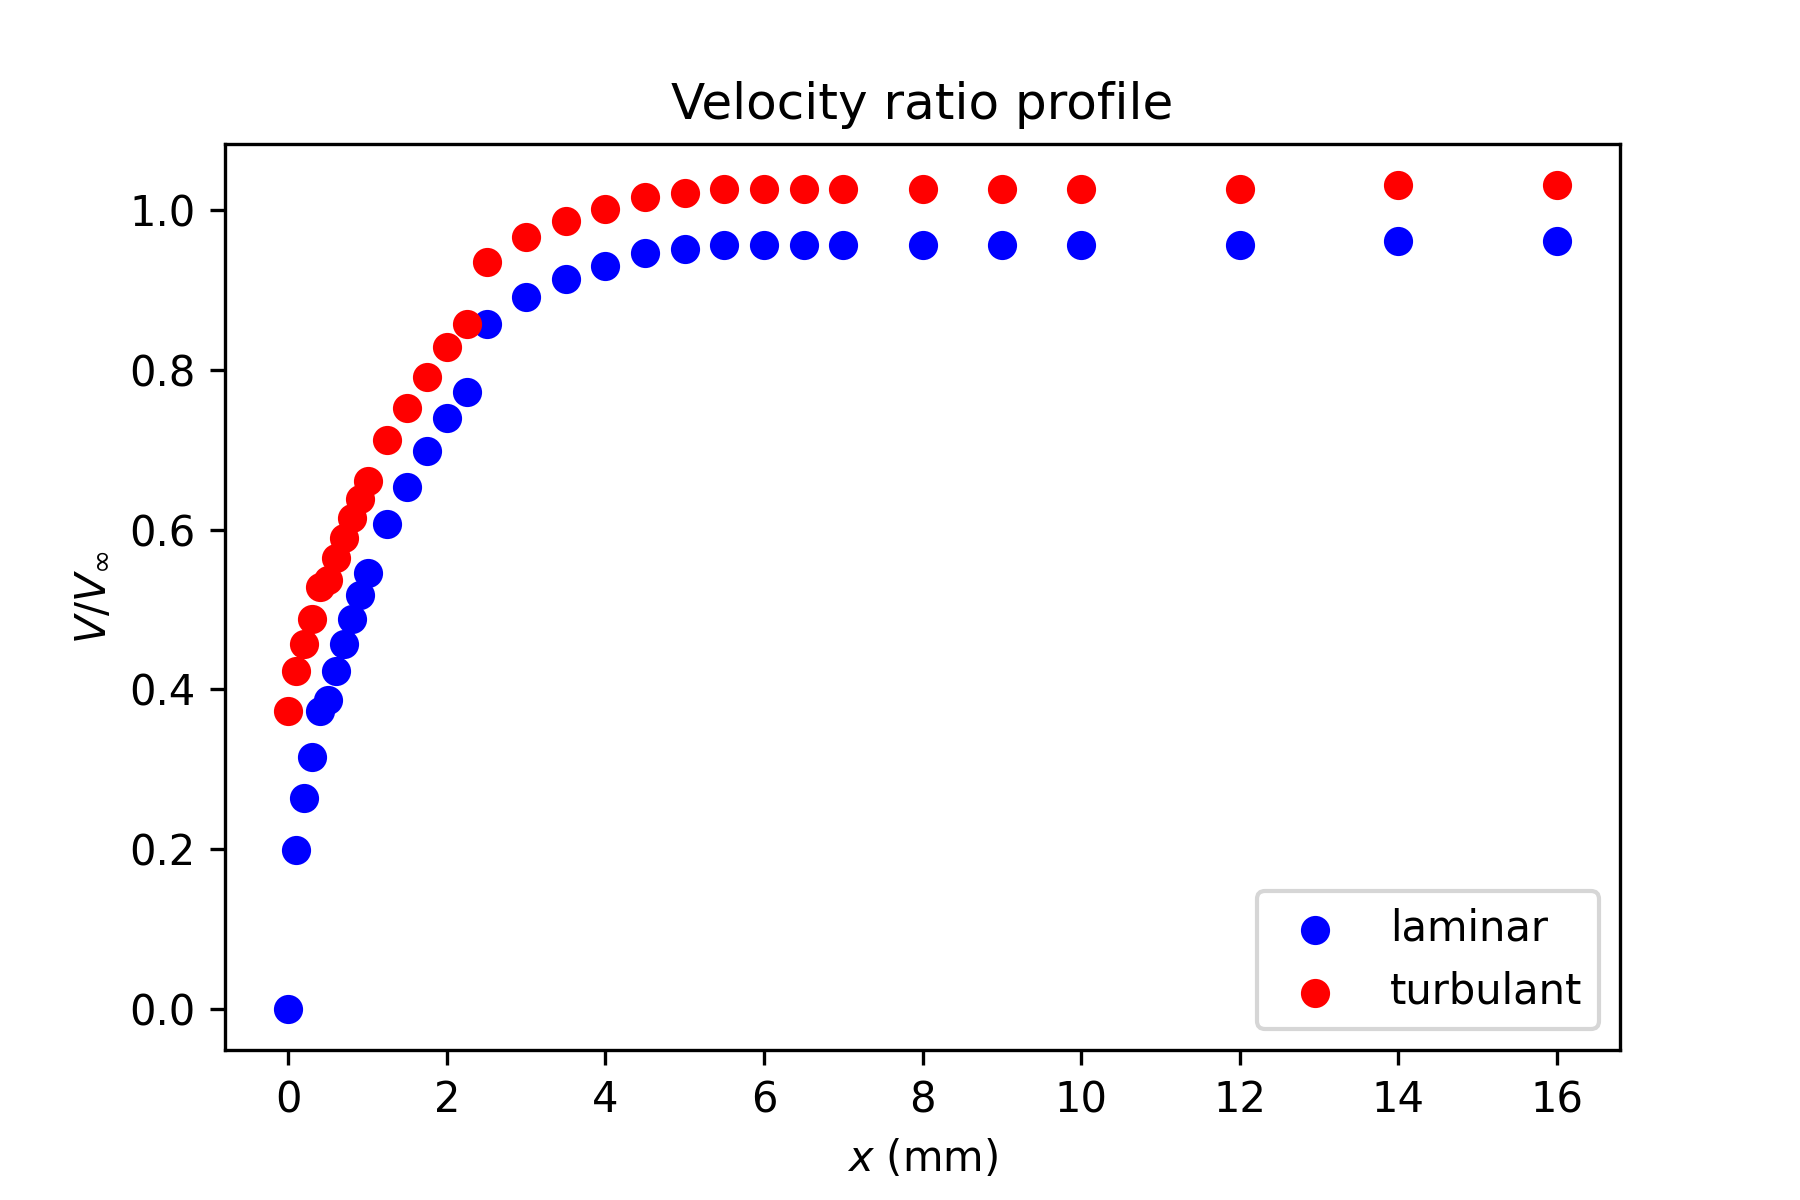
\includegraphics[width=1\textwidth]{velocity_profiles.png}
\caption{\label{fig:velocity_profiles} Graph of the laminar and turbulant flow profiles}
\end{figure}

\begin{figure}[H]
\centering
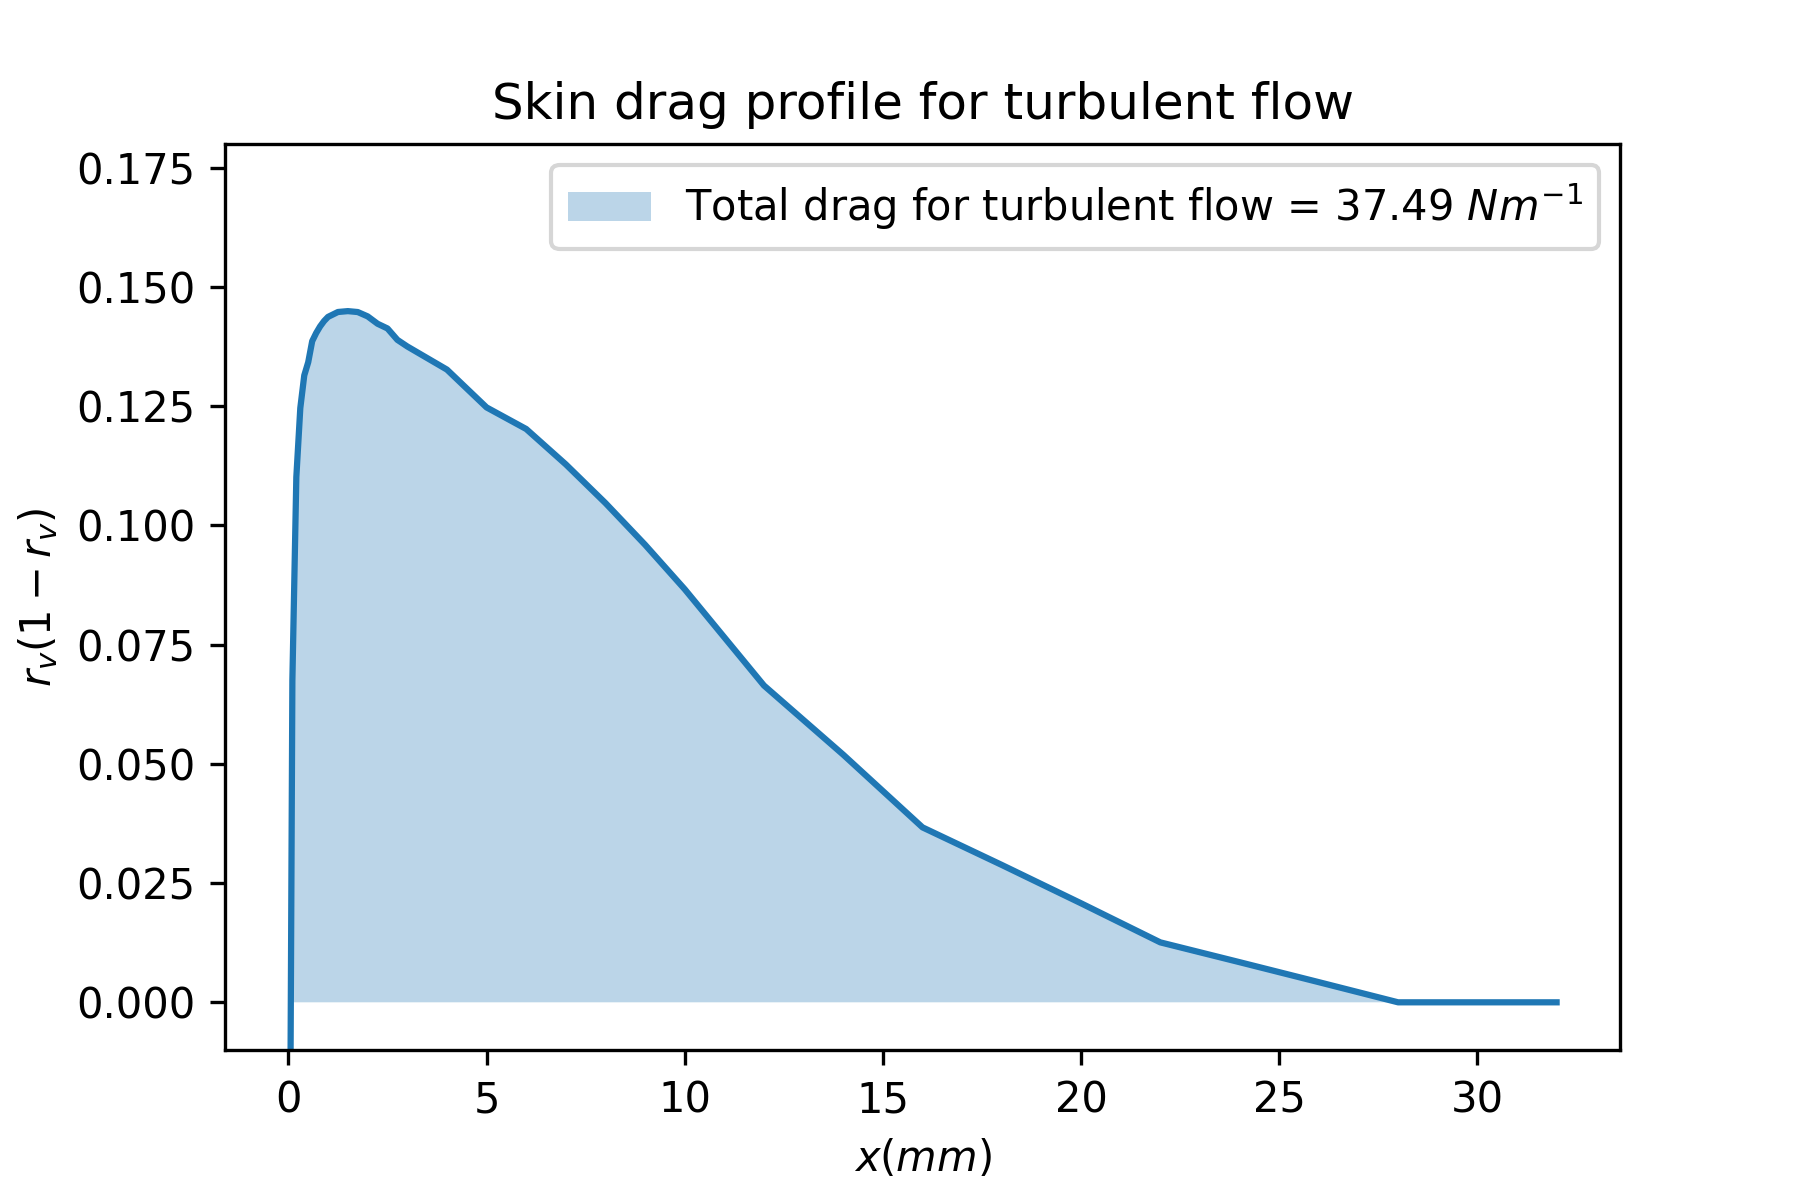
\includegraphics[width=1\textwidth]{turbulent_drag.png}
\caption{\label{fig:turbulent_drag} Graph of the turbulent skin drag profile and total drag force per unit height of wall from equation (5)}
\end{figure}

\begin{figure}[H]
\centering
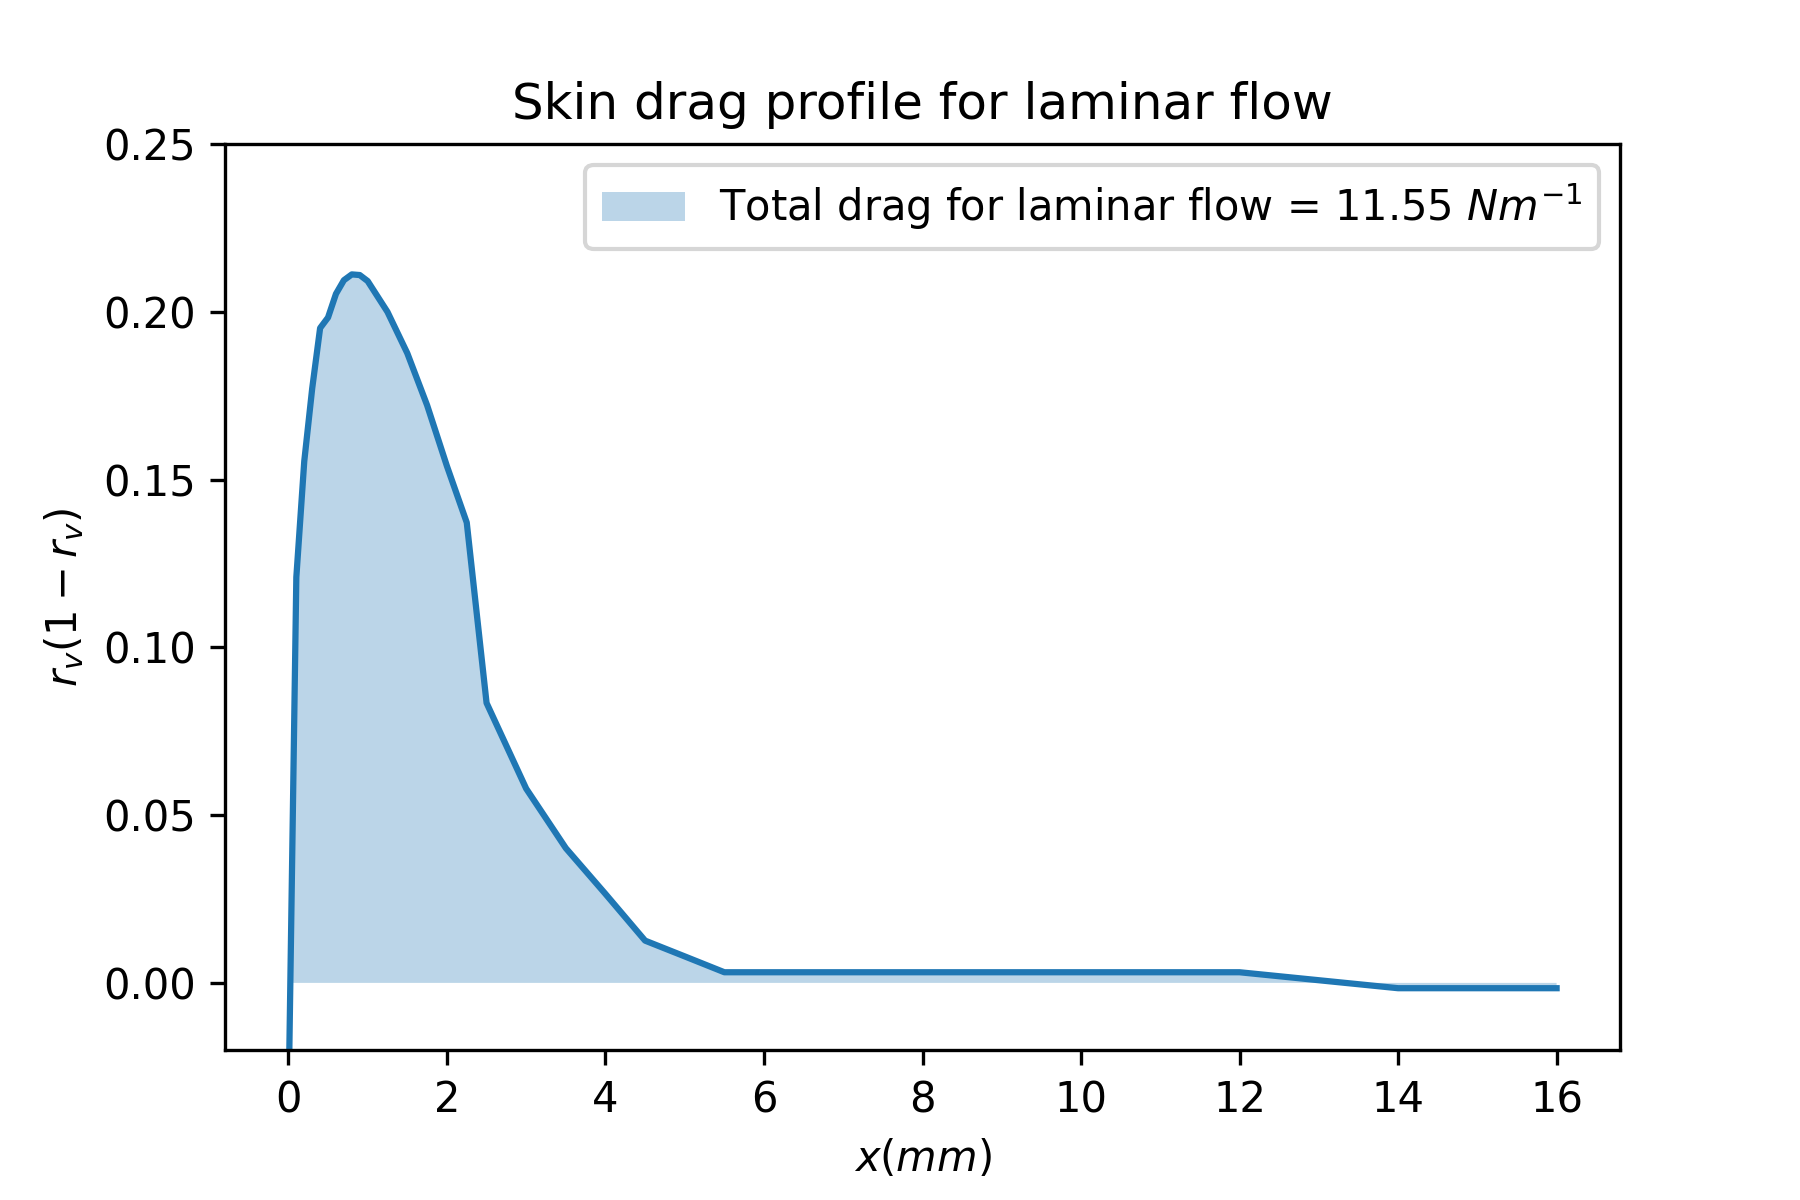
\includegraphics[width=1\textwidth]{laminar_drag.png}
\caption{\label{fig:laminar_drag} Graph of the laminar skin drag profile and total drag force per unit height of wall from equation (5)}
\end{figure}

\subsection{Drag Coefficients}

\begin{figure}[H]
\centering
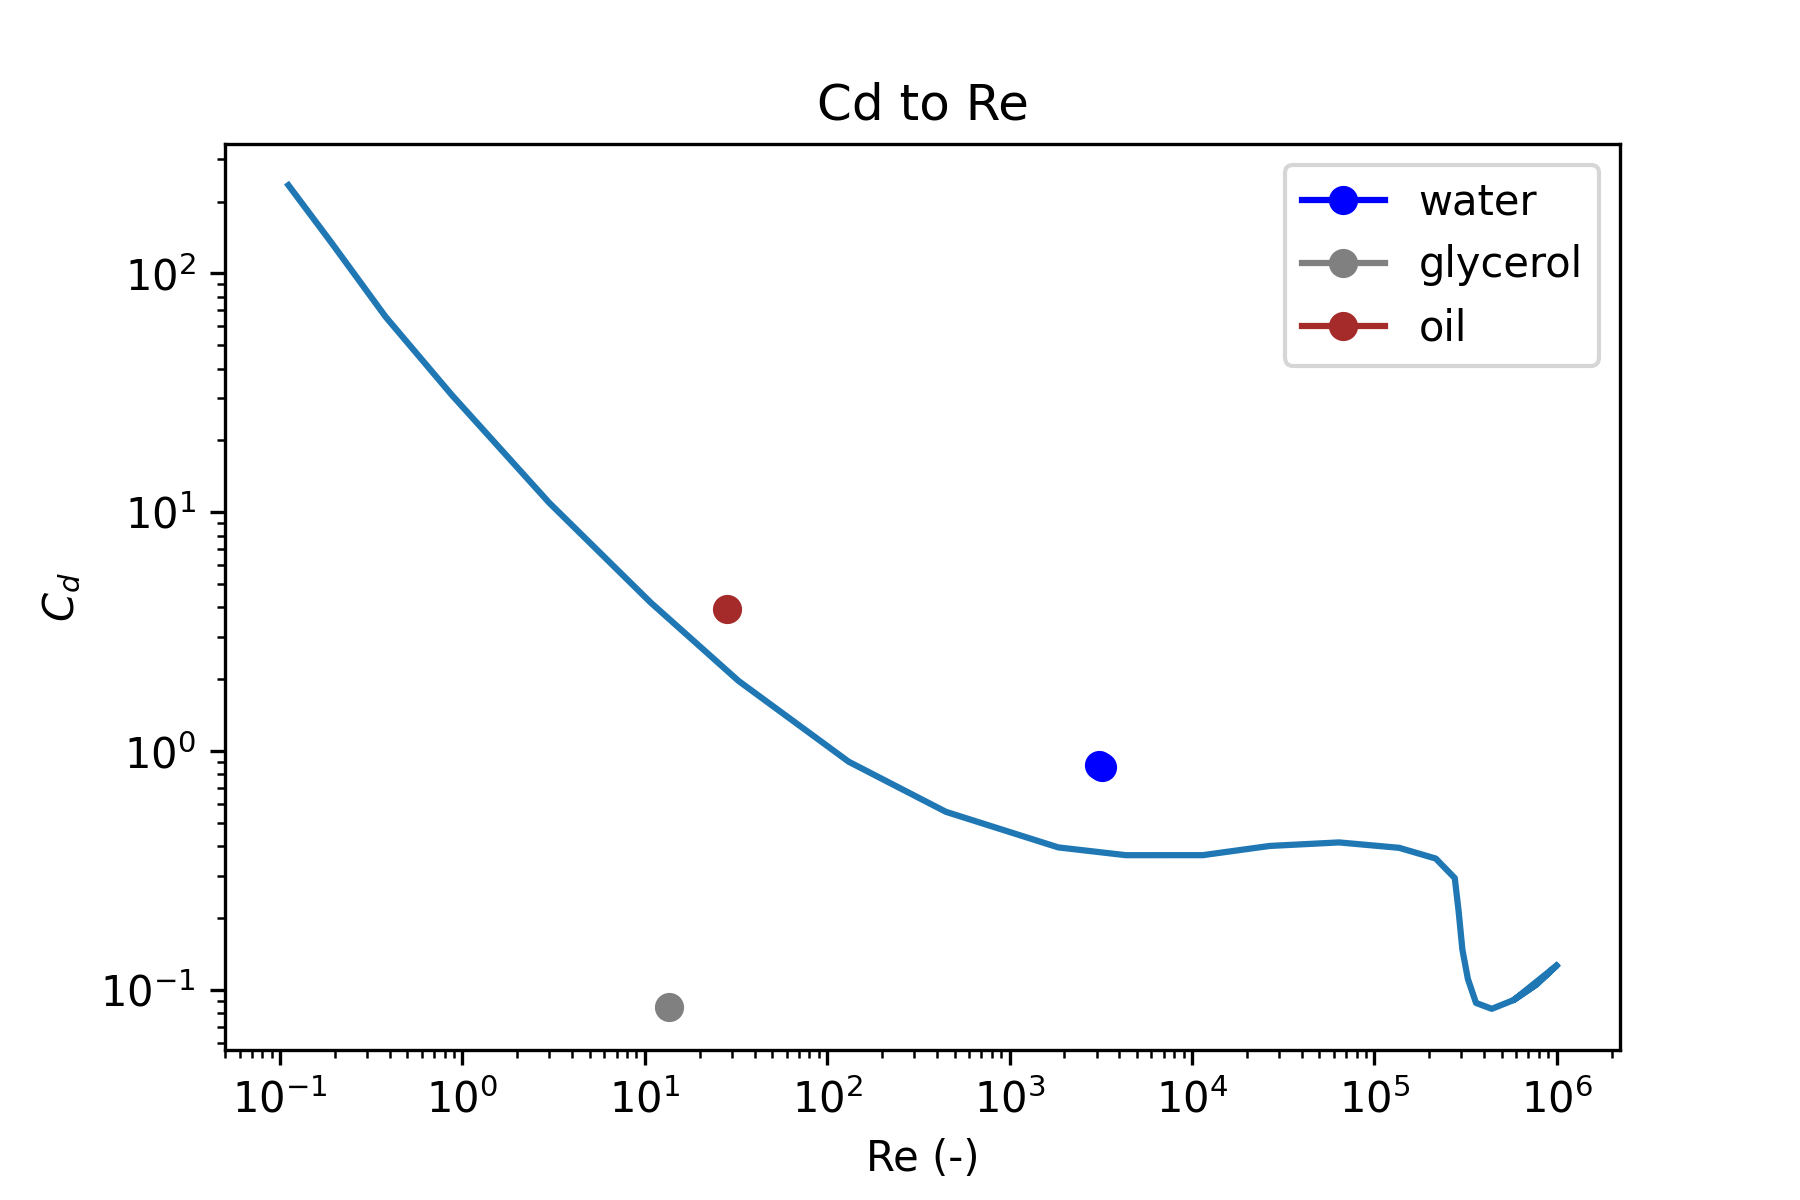
\includegraphics[width=1\textwidth]{CdRe_graph.png}
\caption{\label{fig:CdRe_graph} The drag coefficient of spheres as a function of Re}
\end{figure}

\section{Discussion}

The sudden drop in drag coefficient is due to the boundary layer in front of the sphere becomming thinner and the flow transitions into turbulant 

%interpret results and comment on anomalies

\section{Conclusion}

In conclusion

\end{document}